\chapter{Implementation Results}

% You can title this chapter as \textbf{Preliminary Results} or \textbf{Work Progress} for the progress reports. Present implementation or experimental results here and discuss them.


% ALL SECTIONS IN THIS CHAPTER ARE OPTIONAL. PLEASE CONSULT YOU ADVISOR AND DESIGN YOUR OWN SECTION

% \emph{\textthai{หัวข้อต่าง ๆ ในแต่ละบทเป็นเพียงตัวอย่างเท่านั้น หัวข้อที่จะใส่ในแต่ละบทขึ้นอยู่กับโปรเจคของนักศึกษาและอาจารย์ที่ปรึกษา}}
\section{Introduction}
This chapter provides a comprehensive overview of the results derived from all the implementations undertaken throughout the project. It elaborates on the methodologies employed for testing, including a detailed explanation of the processes and techniques used to ensure accuracy and reliability. Additionally, it specifies the sources of information utilized, highlighting their relevance and credibility in supporting the project objectives. Furthermore, the chapter outlines the evaluation criteria applied to each test, offering a clear framework for assessing the effectiveness and success of the implemented solutions. This structured approach ensures transparency and provides a solid foundation for interpreting the outcomes of the project.

\section{Phase 1}
    \subsection{Prompt Tuning}
    To evaluate the overall performance of the Query Assistance prompt, prompt tuning is conducted. This approach is prioritized due to the agent's heavy reliance on prompts. Ensuring the effectiveness of the prompt is critical, as it guides the agent to operate in alignment with its intended purpose.

    A comprehensive list of scenarios has been tested to assess the system's performance. For each scenario, corresponding test cases are developed and categorized into three levels of difficulty: easy, medium, and hard. For smaller scenarios, a reduced number of test cases is included. Additionally, the weight of these smaller scenarios in the overall performance evaluation is halved relative to the number of cases. The success rate for each scenario is then analyzed to provide insights into the system's effectiveness. Four versions of the prompt have been developed to optimize the performance of the Query Assistance system.
    \begin{itemize}
        \item The first version outlines general requirements for the Query Assistance system, including tasks such as adjusting queries to align with the specified database, adding limits, and other foundational functionalities.
        \item The second version was refined based on extensive testing across various cases. Observations revealed that the system handled subqueries poorly. To address this, the prompt was updated to emphasize handling subqueries effectively and managing specific scenarios, such as cases where no data is returned.
        \item The third version focuses on improving clarity and usability by reorganizing the prompt into distinct sections. This structural adjustment aims to facilitate the agent's ability to process and execute tasks more efficiently.
        \item The fourth version introduces a structured output format to enhance consistency and readability. Additionally, it emphasizes the importance of preserving correct table and column names, ensuring that these elements remain unaltered during query adjustments.
        \item The fifth version was developed after deploying the system for user access and making adjustments based on the results obtained and the analysis of error causes. The first issue we identified was its inability to properly handle arrays. Additionally, we observed that it did not consistently include basic optimizations, such as adding the partition column. To address these issues, we incorporated them into the prompt, which subsequently improved overall performance.
    \end{itemize}
    \begin{table}[H]
        \centering
        \caption[Result of Prompt Tuning]{Result of Prompt Tuning}
        \label{fig:prompt-tuning}
        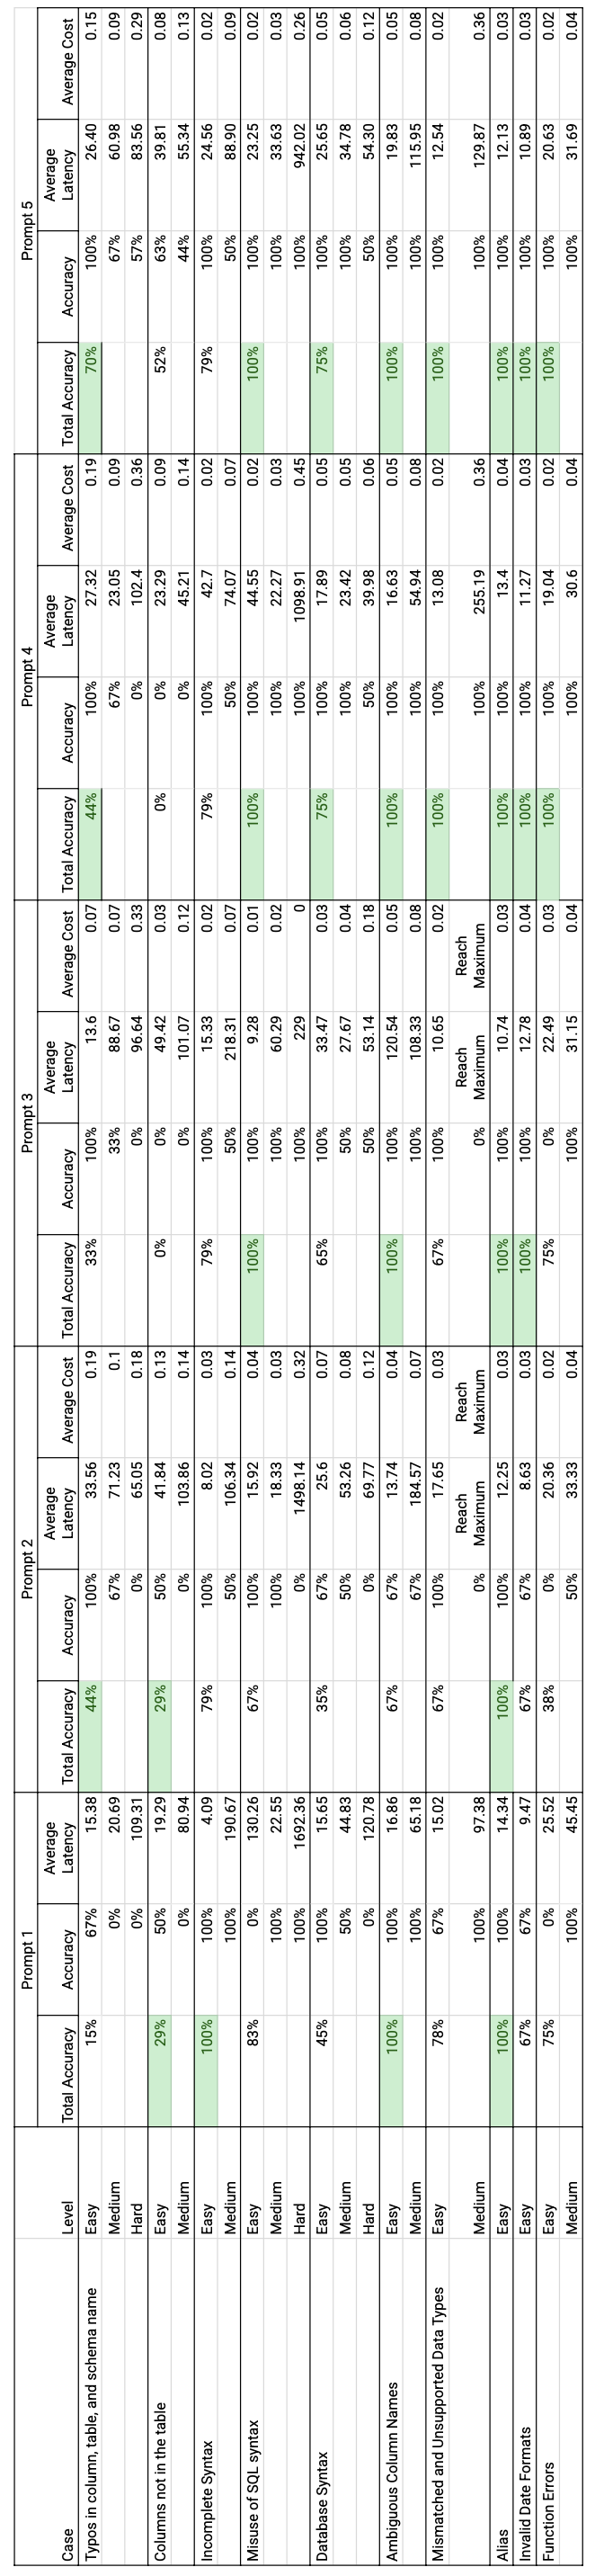
\includegraphics[width=6cm]{chapters/4/figures/prompt.png}
    \end{table}
    \textbf{Metrics for Evaluating}
    \begin{itemize}
        \item Latency is defined as the duration between the initiation of an API request and the receipt of the corresponding response. This metric is critical for evaluating the performance and responsiveness of the system, as it directly impacts user experience and operational efficiency. A lower latency indicates a faster and more efficient system, which is often a key objective in optimizing API interactions.
        \item Cost is determined using the get\_openai\_callback function provided by the LangChain Community (langchain\_community.callbacks). This function calculates the token usage and associated cost based on the specific OpenAI model employed. By leveraging this tool, we can accurately monitor and manage the financial implications of utilizing different models, ensuring cost-effectiveness while maintaining the desired level of performance and accuracy.
        \item Accuracy is assessed by analyzing the similarity and correctness of the SQL query results. This involves comparing the output against expected results to ensure they are aligned and capable of resolving the identified issue. A high level of accuracy is essential for maintaining the reliability and effectiveness of the system, as it ensures that the generated solutions are both relevant and actionable. This metric serves as a key indicator of the system's ability to address complex problems and deliver meaningful outcomes.
    \end{itemize}
\pagebreak